\documentclass[10pt,a4paper]{article}
\usepackage[utf8]{inputenc}
\usepackage{amsmath}
\usepackage{amsfonts}
\usepackage{amssymb}
\usepackage{hyperref}
\usepackage{listings}
\usepackage[many]{tcolorbox}
\tcbuselibrary{listings}

\newtcblisting{mylisting}{
  listing only,
  hbox,
  colframe=cyan,
  colback=cyan!10,
  listing options={
    basicstyle=\small\ttfamily,
    breaklines=true,
    columns=fullflexible
  },
}

%hyperlink parameters
\hypersetup{
    colorlinks=true,
    linkcolor=blue,
    filecolor=magenta,      
    urlcolor=cyan,
    pdftitle={Overleaf Example},
    pdfpagemode=FullScreen,
    }
\urlstyle{same}

\author{Sarah}
\title{Coding in Fortran with Jupyter Notebook}
%\date{today}

\begin{document}
\maketitle{}
\newpage

\section{Part 1: Introduction}
This document summarizes the different stages to run a Fortran code using Colab in the first part. In a second part, how to run it using OpenACC.\\
The aim of this report is to record a guide but also to list some errors encountered doing so.
\section{Part 2: Running a Fortran code in Colab}
\subsection{Installing Colab}
In our particular case, we want to work with Fortran. To do so, we have to set up Colab to run with this specific language.
First and foremost, we should install a Fortran kernel. One can refer \href{https://github.com/ZedThree/jupyter-fortran-kernel}{here} to get more details about the process.\\

\subsubsection{Cloning}
\noindent The first step is to clone the jupyter-fortran-kernel from github.
\begin{lstlisting}[language=bash]
$ git clone git@github.com:ZedThree/jupyter-fortran-kernel.git
\end{lstlisting}

\subsubsection{Installation}
Once the folder downloaded, one shlould install the kernel fortran using:
\begin{lstlisting}[language=bash]
$ pip install -e --user jupyter-fortran-kernel
\end{lstlisting}

\noindent Then, launch the following commands:
\begin{lstlisting}[language=bash]
$ cd jupyter-fortran-kernel
$ jupyter-kernelspec install fortran_spec/
\end{lstlisting}
You should get the message when the installation is completed:
\begin{lstlisting}[language=bash]
[InstallKernelSpec] Installed kernelspec fortran_spec in /home/saras/.local/share/jupyter/kernels/fortran_spec
\end{lstlisting}

\subsubsection{Errors Management}
\textbf{SSH key associated to remote}\\
Here an error occured related to the permission. One should then check the access rights.\\
Here the error message:\begin{lstlisting}[language=bash]
Cloning into 'jupyter-fortran-kernel'...
git@github.com: Permission denied (publickey).
fatal: Could not read from remote repository.
Please make sure you have the correct access rights
and the repository exists.
\end{lstlisting}
Problem solved: the SSH key existing in the local machine was not associated with my Github account.\\
Check this \href{https://docs.github.com/en/authentication/connecting-to-github-with-ssh/adding-a-new-ssh-key-to-your-github-account}{link} to add the key to your account.
\vspace{0.2cm}\\
\textbf{Pip install option --user}\\
The package installer pip for Python is used to launch the installation.
\begin{lstlisting}[language=bash]
$ pip install -e --user jupyter-fortran-kernel
\end{lstlisting}

\noindent In my case, this commands gave an error:
\begin{lstlisting}
ERROR: --user is not a valid editable requirement. It should either be a path to a local project or a VCS URL (beginning with svn+, git+, hg+, or bzr+).
\end{lstlisting}
To overcome this, one can simply switch the two options of the pip install command such as:
\begin{lstlisting}[language=bash]
$ pip install --user -e jupyter-fortran-kernel
\end{lstlisting}
\vspace{0.2cm}
\textbf{Launching from terminal}\\
After installing the kernel, we can launch the notebook by running the command jupyter-notebook from the terminal.\\
An error can occur:
\begin{lstlisting}[language=bash]
Access to the file was denied .local/share/jupyter/runtime/nbserver-113142-open.html is not readable
\end{lstlisting}
The problem can happen for versions of notebook $>$ 5.7.2, a security feature measure was added that prevented the authentication token used to launch the browser from being visible. This feature makes it difficult for other users on a multi-user system from running code in your Jupyter session as you.\\
A way to solve this problem can be found \href{https://stackoverflow.com/questions/70753768/jupyter-notebook-access-to-the-file-was-denied}{here}.


\subsection{Compiling \& Executing}
In our particular case, it is relevant now to introduce Fortran. Because it is a high-level computer langage and more important it is a compiled langage. That means it cannot be run until the compilation stage.\\
In the other hand, we work in the Jupyter Notebook which is an interactive environment and interpreted oriented.\\
A way to overcome this incompatibility is to write the Fortran code inside a file, then, to execute the file as a script.
To do so, the fortran kernel is no longer required, and we need to switch to the python kernel to use what we call Magics. They are powerful tools provided by the IPython kernel.
\begin{itemize}

\item
\begin{lstlisting}[language=bash]
%%writefile
\end{lstlisting}
Writes the content of the cell into a file that should be specify right after the magics command
\begin{mylisting}
%%writefile get_age.f95

program get_age
    real :: year, age
    print *, 'What year were you born?'
    read *, year
    age = 2022 - year
    print *, 'Your age is', age
end program get_age
\end{mylisting}
\item 
\begin{lstlisting}[language=bash]
%%bash
\end{lstlisting}
Allow us to run cells with bash.
\begin{mylisting}
%%bash

gfortran -ffree-form get_age.f95
./a.out
1984
\end{mylisting}
\end{itemize}
\subsection{Results}

\section{Part 2: OpenACC on Colab}
Most of what will be presented here comes from this \href{https://colab.research.google.com/github/ENCCS/OpenACC-CUDA-beginners/blob/colab_gcc/examples/openACC_CUDA_colab.ipynb}{tutorial}.
\subsection{Starting}
Colab is a 
\begin{lstlisting}
!nvidia-smi
\end{lstlisting}
Here the outcome of this command:
\begin{center}
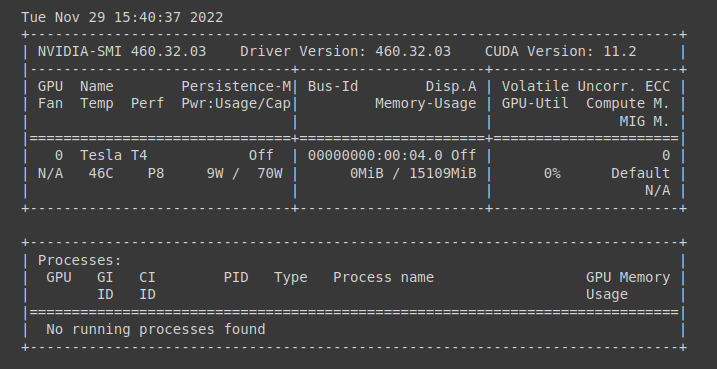
\includegraphics[scale=0.8]{nvidiasmi.png}
\end{center}

\end{document}